\documentclass{article}
\usepackage{helvet}
\usepackage{geometry}
\usepackage{graphicx}
\usepackage{amsmath}
\usepackage{hyperref}
\usepackage{xcolor}
\usepackage{titlesec}
\usepackage{microtype} % Prevents overfull hboxes by better text wrapping
\geometry{margin=1in}
\usepackage{subcaption}
\usepackage{listings}
\usepackage{color}
% Define colors for code syntax highlighting
\definecolor{codeblue}{rgb}{0.13, 0.13, 0.7}
\definecolor{codegreen}{rgb}{0, 0.5, 0}
\definecolor{codegray}{rgb}{0.5, 0.5, 0.5}
\definecolor{codepurple}{rgb}{0.58, 0, 0.82}

\lstdefinestyle{mystyle}{
    backgroundcolor=\color{white},   
    commentstyle=\color{codegreen},
    keywordstyle=\color{codeblue},
    numberstyle=\tiny\color{codegray},
    stringstyle=\color{codepurple},
    basicstyle=\ttfamily\footnotesize,
    breaklines=true,                 
    captionpos=b,                    
    keepspaces=true,                 
    numbers=left,                    
    numbersep=5pt,                  
    showspaces=false,                
    showstringspaces=false,
    showtabs=false,                  
    tabsize=2
}

\lstset{style=mystyle}

% Define colors
\definecolor{primary}{RGB}{0, 102, 204} % Blue color
\definecolor{IITBBlue}{RGB}{0, 51, 102} % IIT Bombay's signature blue

\usepackage{cite}
\usepackage{amsmath,amssymb,amsfonts}
\usepackage{algorithmic}
\usepackage{graphicx}
\usepackage{textcomp}
\usepackage{xcolor}
\usepackage{hyperref}
\usepackage{placeins}
\usepackage{graphicx}
\usepackage{subcaption}
\usepackage{physics}




\def\BibTeX{{\rm B\kern-.05em{\sc i\kern-.025em b}\kern-.08em
    T\kern-.1667em\lower.7ex\hbox{E}\kern-.125emX}}


\title{Tutorial Set 3, Problem 2: EE 338, Spring 2024-25}
\author{
\IEEEauthorblockN{
    \begin{tabular}{cccc}
        \begin{minipage}[t]{0.23\textwidth}
            \centering
            Anupam Rawat\\
            IIT Bombay\\
            22b3982@iitb.ac.in
        \end{minipage} & 
        \begin{minipage}[t]{0.23\textwidth}
            \centering
            Rishabh Bhardwaj\\
            IIT Bombay\\
            22b3962@iitb.ac.in
        \end{minipage} & 
        \begin{minipage}[t]{0.23\textwidth}
            \centering
            Jatin Kumar\\
            IIT Bombay\\
            22b3922@iitb.ac.in
        \end{minipage} \\
        \\ 
    \end{tabular}
}
}

\date{January 18, 2025}


\usepackage{amsmath}
\usepackage{amssymb}
\usepackage{hyperref}
\usepackage{ulem,graphicx}
\usepackage[margin=0.5in]{geometry}

\begin{document}
\maketitle

\\

\begin{enumerate}
    \item Consider the following two discrete time LSI systems:
    \begin{enumerate}
        \item y[n] = \{ x[n] + x[n-1] \} / 2
        \item y[n] = \{ x[n] - x[n-1] \} / 2
        \begin{enumerate}
            \item Obtain their impulse responses; $h_a[n]$ and $h_b[n]$ respectively
            \item Obtain their frequency responses; $H_a(\omega)$ and $H_a(\omega)$ respectively
            \item Let the input sequence x[n] = cos$\omega_0$n be applied to each of these systems. Here $\omega_0$ is between 0 and $\pi$. Obtain the output sequences $y_a$[n] and $y_b$[n] respectively without using the impulse response or frequency response. You may use trigonometric identities. e.g. cos A + cos B = 2 cos .... cos.... etc.
            \item Now correlate your result of part (iii) with that of part (ii).
            \item Find the inverse Discrete Time Fourier Transforms (inverse DTFTs) of $H_a(\omega)$ and $H_b(\omega)$: verify that they are indeed $h_a$[n] and $h_b$[n] respectively.
            \item Obtain and sketch the magnitude and phase of $H_a(\omega)$ and $H_b(\omega)$ as a function of $\omega$ for the region $\omega$: 0 to $\pi$. Approximately speaking, what kind of filters can we call them?
        \end{enumerate}
    \end{enumerate}
        
    \\
        \makebox[0pt][l]{\hspace{-7pt}\textit{Soln:}} % Aligns "Answer:" to the left
    \\
    
    \begin{enumerate}
        \item 
        \begin{enumerate}
            \item 
                \[
                    h_a[n] = \frac{\delta[n] + \delta[n-1]}{2} 
                        = 
                        \begin{cases} 
                        \frac{1}{2} & \text{if } n = 0 \text{ or } n = 1, \\
                        0 & \text{otherwise.}
                        \end{cases}
                \]
            \item 
                \[
                    H_a(\omega) = \Sigma_nh[n]e^{-j\omega n} = \Sigma_n(\frac{\delta[n] + \delta[n-1]}{2})e^{-j\omega n}
                \]
                \[
                    H_a(\omega) = \frac{ \delta[0]e^{-j\omega (0)} }{2} + \frac{ \delta[1-1]e^{-j\omega (1)} }{2} = \frac{1}{2} + \frac{1}{2}e^{-j\omega}
                \]
            \item
                \[
                    x[n] = cos(\omega_0n)
                \]
                Substituting the above given x[n] in the equation of y[n] we get:
                \[
                    y_a[n] = \frac{ cos(\omega_0n) + cos(\omega_0(n-1)) }{2}
                \]
                We also know that $cos(A) + cos(B) = 2 cos\left(\frac{A + B}{2} \right) \cdot cos\left( \frac{A-B}{2} \right)$
                \[
                    y_a[n] = cos\left(\omega_0( n - \frac{1}{2} )\right)cos\left(\frac{\omega_0}{2} )\right)
                \]
                Also, since: 
                \[
                    cos(\omega_0 n) = \frac{e^{-j\omega_0n} + e^{j\omega_0n}}{2}
                \]
                The expression of $y_a[n]$ in the form of cos(A) + cos(B) can be expressed as:
                \[
                    y_a[n] = \left( \frac{ e^{-j\omega_0n} + e^{j\omega_0n}}{4} \right) + \left( \frac{ e^{-j\omega_0(n-1)} + e^{j\omega_0(n-1)}}{4} \right)
                \]
                \[
                    y_a[n] = \left( \frac{ e^{-j\omega_0n} + e^{-j\omega_0(n-1)}}{4} \right) + \left( \frac{ e^{j\omega_0n} + e^{j\omega_0(n-1)}}{4} \right)
                \]
                \[
                    y_a[n] = \frac{e^{-j\omega_0n}}{4} \left( 1 + e^{j\omega_0} \right) + \frac{e^{j\omega_0n}}{4} \left( 1 + e^{-j\omega_0} \right)
                \]
            \item
                Discrete Time Fourier Transform of a Discrete Signal a[n] is given by:
                \[
                    \mathcal{F}\{a[n]\} = \Sigma_ka[k]e^{-j\omega k}
                \]
                DTFT of $y_a[n]$:
                \[
                    \mathcal{F}\{y_a[n]\} = Y_a(\omega) = \frac{1 + e^{j\omega_0}}{4} \cdot e^{-j\omega_0n}\cdot e^{-j\omega n} + \frac{1 + e^{-j\omega_0}}{4} \cdot e^{j\omega_0n}\cdot e^{-j\omega n}
                \]
                \[
                    Y_a(\omega) = \frac{1 + e^{-j\omega_0}}{4} \cdot \delta[\omega-\omega_0] + \frac{1 + e^{j\omega_0}}{4} \cdot \delta[\omega+\omega_0]
                \]
                DTFT of x[n]:
                \[
                    \mathcal{F}\{x[n]\} = X(\omega) = \Sigma_n\left(\frac{ e^{-j\omega_0 n} + e^{j\omega_0 n}}{2} \right)\cdot e^{-j\omega n}
                \]

                In the time domain, the convolution of x[n] and h[n] yields the output. To get the output in the frequency domain, we simply have to multiply X($\omega$) and H($\omega$):
                \[
                    Y_a(\omega) = X_a(\omega)\cdot H_a(\omega) = \left( \frac{\delta[\omega-\omega_0]}{2} + \frac{\delta[\omega+\omega_0]}{2} \right) \cdot \frac{1 + e^{-j\omega}}{2}
                \]
                \[
                    Y_a(\omega) = \frac{1 + e^{-j\omega_0}}{4} \cdot \delta[\omega-\omega_0] + \frac{1 + e^{+j\omega_0}}{4} \cdot \delta[\omega+\omega_0]
                \]
                As it can be seen, the above expression matches that of $Y_a(\omega)$, thus we can conclude that the result of part iii. was valid.
            \item
                The Inverse DTFT of a signal is given as:
                \[
                    \mathcal{F}^{-1}\{P(\omega)\} = \frac{1}{2\pi}\int_{-\pi}^{\pi}(\omega)e^{j\omega n}
                \]
                \[
                    \mathcal{F}^{-1}\{H_a(\omega)\} = h_a[n] = \frac{1}{2\pi} \int_{-\pi}^{\pi}H_a(\omega) e^{j\omega n} d\omega
                \]
                \[
                    h_a[n] = \frac{1}{2\pi} \int_{-\pi}^{\pi} \frac{1 + e^{-j\omega}}{2} e^{j\omega n} d\omega = \frac{1}{4\pi} \int_{-\pi}^{\pi} e^{j\omega n} d\omega + \frac{1}{4\pi} \int_{-\pi}^{\pi} e^{j\omega (n-1)} d\omega.
                \]
                It is known that: 
                \[
                    \int_{-\pi}^{\pi} e^{j\omega k} d\omega =
                    \begin{cases}
                        2\pi, & \text{if } k = 0, \\
                        0, & \text{if } k \neq 0,
                    \end{cases}
                \]
                we evaluate the two terms:
                \[
                    \begin{array}{cc}
                        \frac{1}{4\pi} \int_{-\pi}^{\pi} e^{j\omega n} d\omega =
                        \begin{cases}
                            \frac{1}{2}, & \text{if } n = 0, \\
                            0, & \text{if } n \neq 0,
                        \end{cases}
                        &
                        \frac{1}{4\pi} \int_{-\pi}^{\pi} e^{j\omega (n-1)} d\omega =
                        \begin{cases}
                            \frac{1}{2}, & \text{if } n = 1, \\
                            0, & \text{if } n \neq 1.
                        \end{cases}
                    \end{array}
                \]
                Thus, the $h_a$[n] can be written as:
                \[
                    h_a[n] =
                        \begin{cases} 
                        \frac{1}{2} & \text{if } n = 0 \text{ or } n = 1, \\
                        0 & \text{otherwise.}
                        \end{cases}
                \]
                \[
                    h_a[n] =\frac{\delta[n] + \delta[n-1]}{2}.
                \]
                which is the same as the result obtained in part i.
            \item 
                We can express the $H_a(\omega)$ in terms of phasor:
                \[
                    H_a(\omega) = \frac{1 + e^{-j\omega}}{2} = \frac{1 + cos(\omega)}{2} - j \frac{sin(\omega)}{2}
                \]
                Phase of a phasor is given by the tan inv of ratio of img component to the real one:
                \[
                    \theta = \tan^{-1} \left( \frac{-sin(\omega)}{1 + cos(\omega)} \right)
                \]
                Magnitude of a phasor is given by sqrt of sum of square of the two components:
                \[
                    magnitude = \sqrt{\left( 1 + cos(\omega) + \frac{cos^2(\omega)}{4} \right) + \frac{sin^2(\omega)}{4}} = \sqrt{1 + \frac{1}{4} + cos(\omega)} = \sqrt{\frac{5}{4} + cos(\omega)}
                \]
                By looking at Magnitude Plot we can say that this is smoothening: averages current and previous response, acting like a \textbf{Low Pass Filter}
                \begin{figure}[h!]
    \centering
    \begin{subfigure}[b]{0.45\linewidth}
        \centering
        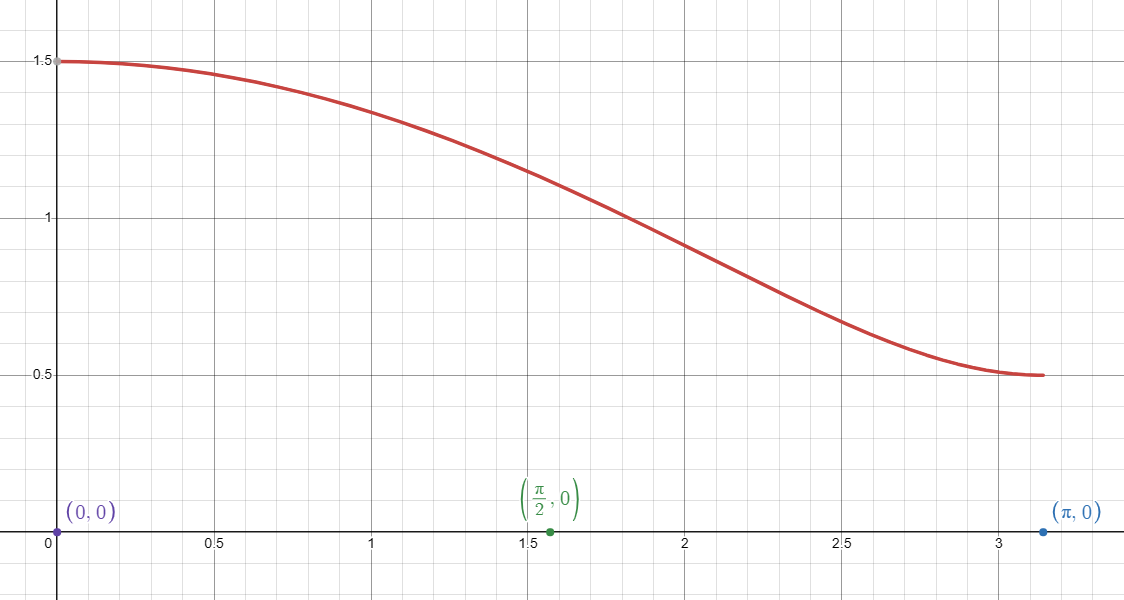
\includegraphics[width=\linewidth]{./images/Tutorial_Set_3_Ques_2_part_a_subpart_vi_magnitude.png}
        \caption{Plot of magnitude of $H_a(\omega)$}
        \label{fig:magnitude_ha}
    \end{subfigure}
    \hfill
    \begin{subfigure}[b]{0.45\linewidth}
        \centering
        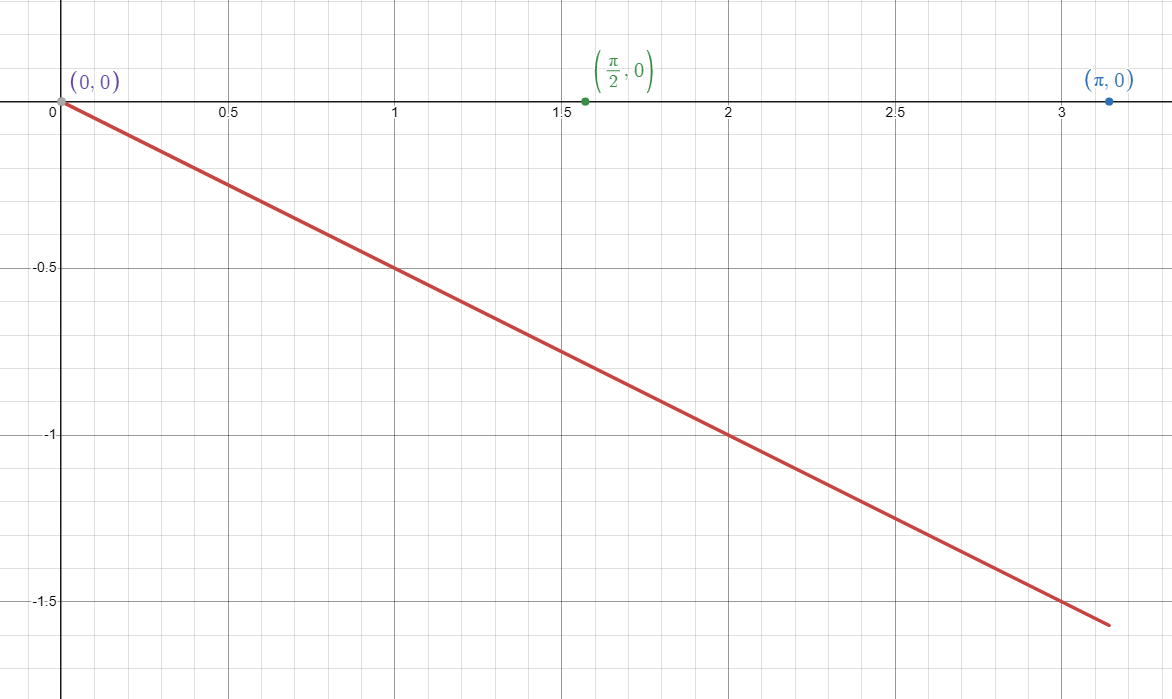
\includegraphics[width=\linewidth]{./images/Tutorial_Set_3_Ques_2_part_a_subpart_vi_phase.png}
        \caption{Plot of phase of $H_a(\omega)$}
        \label{fig:phase_ha}
    \end{subfigure}
    \caption{Plots of $H_a(\omega)$}
    \label{fig:ha_omega}
\end{figure}
        \end{enumerate}



  
        \item 
        \begin{enumerate}
            \item 
                \[
                    h_b[n] = \frac{\delta[n] - \delta[n-1]}{2} 
                        = 
                        \begin{cases} 
                        \frac{1}{2} & \text{if } n = 0, \\
                        \frac{-1}{2} & \text{if } n = 1, \\
                        0 & \text{otherwise.}
                        \end{cases}
                \]
            \item 
                \[
                    H_b(\omega) = \Sigma_nh[n]e^{-j\omega n} = \Sigma_n(\frac{\delta[n] - \delta[n-1]}{2})e^{-j\omega n}
                \]
                \[
                    H_b(\omega) = \frac{ \delta[0]e^{-j\omega (0)} }{2} - \frac{ \delta[1-1]e^{-j\omega (1)} }{2} = \frac{1}{2} - \frac{1}{2}e^{-j\omega}
                \]
            \item
                \[
                    x[n] = cos(\omega_0n)
                \]
                Substituting the above given x[n] in the equation of y[n] we get:
                \[
                    y_b[n] = \frac{ cos(\omega_0n) - cos(\omega_0(n-1)) }{2}
                \]
                We also know that $cos(A) - cos(B) = 2 sin\left(\frac{A + B}{2} \right) \cdot sin\left( \frac{B-A}{2} \right)$
                \[
                    y_b[n] = sin\left(\omega_0( n - \frac{1}{2} )\right)sin\left((\frac{-\omega_0}{2} )\right)
                \]
                Also, since: 
                \[
                    sin(\omega_0 n) = \frac{e^{-j\omega_0n} - e^{j\omega_0n}}{2j}
                \]




 The expression of $y_b[n]$ in the form of cos(A) - cos(B) can be expressed as:
                \[
                    y_b[n] = \left( \frac{ e^{-j\omega_0n} + e^{j\omega_0n}}{4} \right) - \left( \frac{ e^{-j\omega_0(n-1)} + e^{j\omega_0(n-1)}}{4} \right)
                \]
                \[
                    y_b[n] = \left( \frac{ e^{-j\omega_0n} - e^{-j\omega_0(n-1)}}{4} \right) + \left( \frac{ e^{j\omega_0n} - e^{j\omega_0(n-1)}}{4} \right)
                \]
                \[
                    y_b[n] = \frac{e^{-j\omega_0n}}{4} \left( 1 - e^{j\omega_0} \right) + \frac{e^{j\omega_0n}}{4} \left( 1 - e^{-j\omega_0} \right)
                \]

 \item
                Discrete Time Fourier Transform of a Discrete Signal b[n] is given by:
                \[
                    \mathcal{F}\{b[n]\} = \Sigma_kb[k]e^{-j\omega k}
                \]
                DTFT of $y_b[n]$:
                \[
                    \mathcal{F}\{y_b[n]\} = Y_b(\omega) = \frac{1 - e^{j\omega_0}}{4} \cdot e^{-j\omega_0n}\cdot e^{-j\omega n} + \frac{1 - e^{-j\omega_0}}{4} \cdot e^{j\omega_0n}\cdot e^{-j\omega n}
                \]
                \[
                    Y_b(\omega) = \frac{1 - e^{-j\omega_0}}{4} \cdot \delta[\omega-\omega_0] + \frac{1 - e^{j\omega_0}}{4} \cdot \delta[\omega+\omega_0]
                \]
                DTFT of x[n]:
                \[
                    \mathcal{F}\{x[n]\} = X(\omega) = \Sigma_n\left(\frac{ e^{-j\omega_0 n} + e^{j\omega_0 n}}{2} \right)\cdot e^{-j\omega n} = \frac{\delta[\omega-\omega_0]}{2} + \frac{\delta[\omega+\omega_0]}{2}
                \]

                In the time domain, the convolution of x[n] and h[n] yields the output. To get the output in the frequency domain, we simply have to multiply X($\omega$) and H($\omega$):
                \[
                    Y_b(\omega) = X(\omega)\cdot H_b(\omega) = \left( \frac{\delta[\omega-\omega_0]}{2} + \frac{\delta[\omega+\omega_0]}{2} \right) \cdot \frac{1 - e^{-j\omega}}{2}
                \]
                \[
                    Y_b(\omega) = \frac{1 - e^{-j\omega_0}}{4} \cdot \delta[\omega-\omega_0] + \frac{1 - e^{+j\omega_0}}{4} \cdot \delta[\omega+\omega_0]
                \]
                As it can be seen, the above expression matches that of $Y_b(\omega)$, thus we can conclude that the result of part iii. was valid.

 \item
                The Inverse DTFT of a signal is given as:
                \[
                    \mathcal{F}^{-1}\{P(\omega)\} = \frac{1}{2\pi}\int_{-\pi}^{\pi}(\omega)e^{j\omega n}
                \]
                \[
                    \mathcal{F}^{-1}\{H_b(\omega)\} = h_b[n] = \frac{1}{2\pi} \int_{-\pi}^{\pi}H_b(\omega) e^{j\omega n} d\omega
                \]
                \[
                    h_b[n] = \frac{1}{2\pi} \int_{-\pi}^{\pi} \frac{1 - e^{-j\omega}}{2} e^{j\omega n} d\omega = \frac{1}{4\pi} \int_{-\pi}^{\pi} e^{j\omega n} d\omega - \frac{1}{4\pi} \int_{-\pi}^{\pi} e^{j\omega (n-1)} d\omega.
                \]
                It is known that: 
                \[
                    \int_{-\pi}^{\pi} e^{j\omega k} d\omega =
                    \begin{cases}
                        2\pi, & \text{if } k = 0, \\
                        0, & \text{if } k \neq 0,
                    \end{cases}
                \]
                we evaluate the two terms:
                \[
                    \begin{array}{cc}
                        \frac{1}{4\pi} \int_{-\pi}^{\pi} e^{j\omega n} d\omega =
                        \begin{cases}
                            \frac{1}{2}, & \text{if } n = 0, \\
                            0, & \text{if } n \neq 0,
                        \end{cases}
                        &
                        \frac{1}{4\pi} \int_{-\pi}^{\pi} e^{j\omega (n-1)} d\omega =
                        \begin{cases}
                            \frac{1}{2}, & \text{if } n = 1, \\
                            0, & \text{if } n \neq 1.
                        \end{cases}
                    \end{array}
                \]
                Thus, the $h_b$[n] can be written as:
                \[
                    h_b[n] =
                        \begin{cases} 
                        \frac{1}{2} & \text{if } n = 0, \\
                        \frac{-1}{2} & \text{if } n = 1, \\
                        0 & \text{otherwise.}
                        \end{cases}
                \]
                \[
                    h_b[n] =\frac{\delta[n] - \delta[n-1]}{2}.
                \]
                which is the same as the result obtained in part i.

\item 
                We can express the $H_b(\omega)$ in terms of phasor:
                \[
                    H_b(\omega) = \frac{1 - e^{-j\omega}}{2} = \frac{1 - cos(\omega)}{2} + j \frac{sin(\omega)}{2}
                \]
                Phase of a phasor is given by the tan inv of ratio of img component to the real one:
                \[
                    \theta = \tan^{-1} \left( \frac{-sin(\omega)}{1 - cos(\omega)} \right)
                \]
                Magnitude of a phasor is given by sqrt of sum of square of the two components:
                \[
                    magnitude = \sqrt{\left( 1 - cos(\omega) + \frac{cos^2(\omega)}{4} \right) + \frac{sin^2(\omega)}{4}} = \sqrt{1 + \frac{1}{4} - cos(\omega)} = \sqrt{\frac{5}{4} - cos(\omega)}
                \]

                \begin{figure}[h!]
    \centering
    \begin{subfigure}[b]{0.45\linewidth}
        \centering
        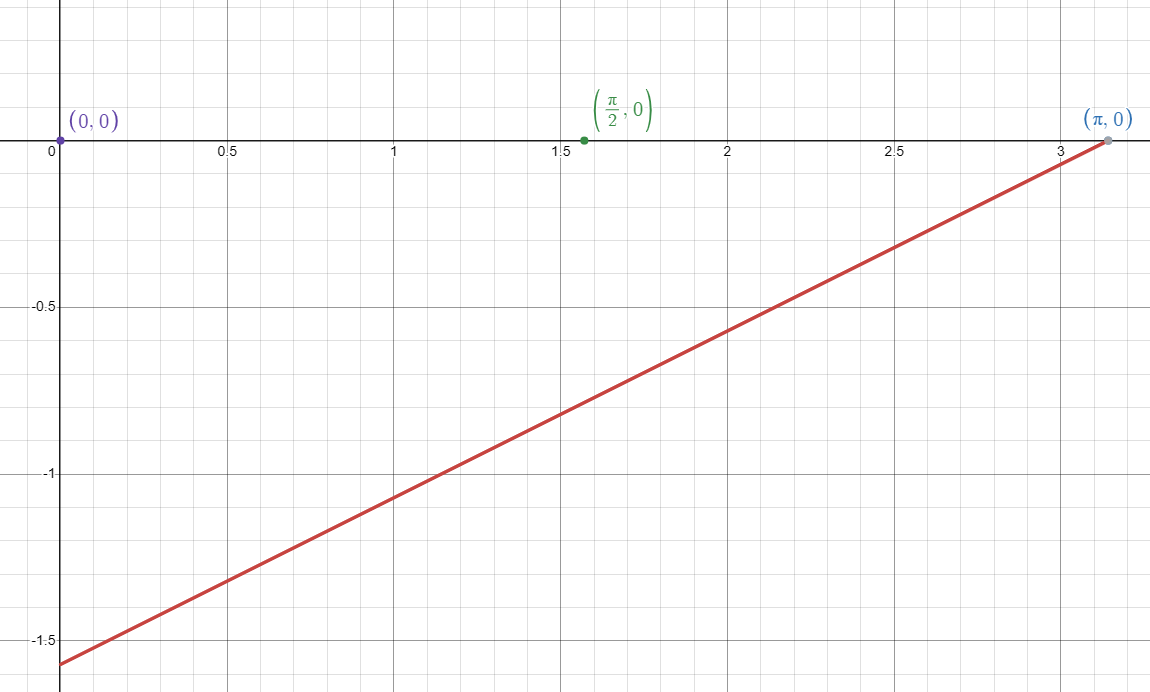
\includegraphics[width=\linewidth]{./images/Tutorial_Set_3_Ques_2_part_b_subpart_vi_phase.png}
        \caption{Plot of phase of $H_b(\omega)$}
        \label{fig:phase}
    \end{subfigure}
    \hfill
    \begin{subfigure}[b]{0.45\linewidth}
        \centering
        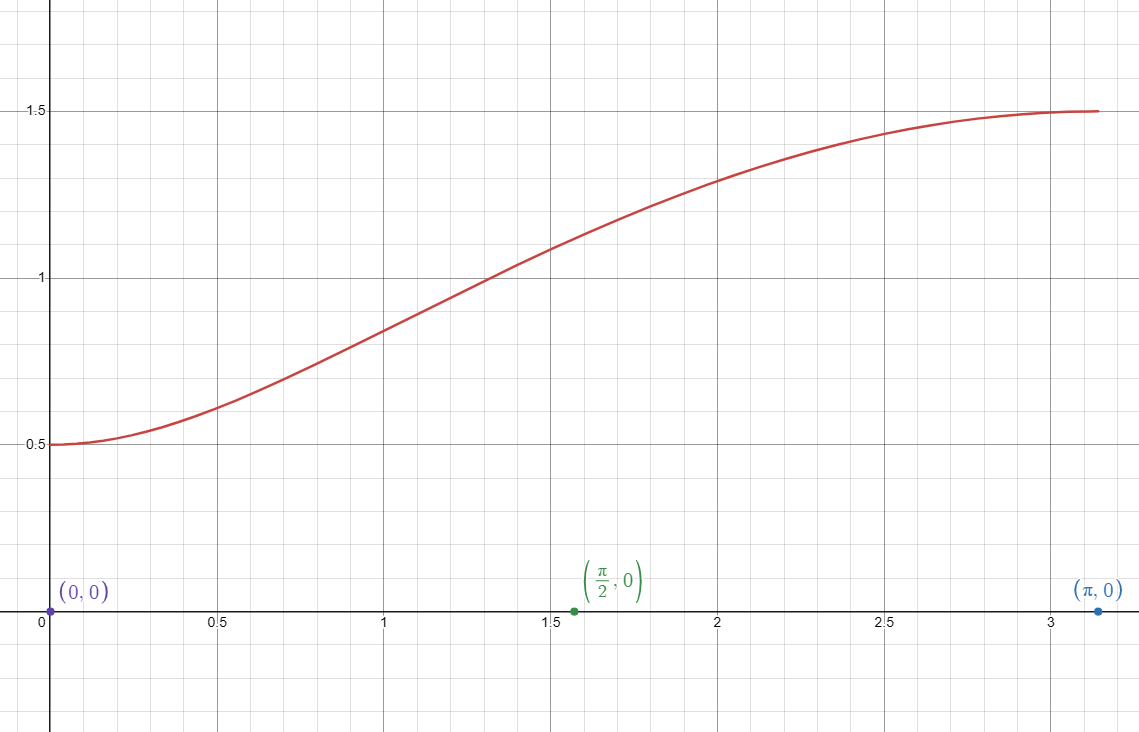
\includegraphics[width=\linewidth]{./images/Tutorial_Set_3_Ques_2_part_b_subpart_vi_magnitude.png}
        \caption{Plot of magnitude of $H_b(\omega)$}
        \label{fig:magnitude}
    \end{subfigure}
    \caption{Plots of $H_b(\omega)$}
    \label{fig:hb_omega}
\end{figure}


                By looking at Magnitude Plot we can say that this is doing \textbf{Edge Detection}, and acting like a \textbf{High Pass Filter}
        \end{enumerate}       
    \end{enumerate}
    
\end{enumerate}
\end{document}

